% update date: 2024.09.04
% 有問題or更新需求可email至: wufish@gmail.com
% 也可以到github留言: https://github.com/coldwufish/NYCU-thesis-template

% 載入會用到的套件, 通常不需要修改這邊的資料
\documentclass[12pt,a4paper,oneside]{book}
\usepackage[ top=2.5cm,bottom=2.5cm,left=3cm,right=2cm ]{ geometry }

\usepackage{subcaption}
\usepackage{caption}

\usepackage[no-math]{fontspec}   %加這個就可以設定字體 
\usepackage{xeCJK}       %讓中英文字體分開設置 
\usepackage[UTF8,fontset=none,scheme=plain]{ctex}
\setCJKmainfont[AutoFakeBold={4}, AutoFakeSlant=0.2]{TW-Kai}
\setmainfont{Times New Roman}
\usepackage{CJKnumb}

\usepackage{indentfirst}
\usepackage{array}
\usepackage{multirow}
\usepackage{amsthm}
\usepackage{amsmath}
\usepackage{amsfonts}
\usepackage{amssymb}
\usepackage{graphicx}
\usepackage{multirow}
\usepackage{setspace}
%\usepackage{cite}
\usepackage{balance}
\usepackage{textcomp}
\usepackage{color}
\usepackage[ampersand]{easylist}
\ListProperties(Hide=100, Hang=true, Progressive=3ex, Style*=$\bullet$ ,
Style2*=\tiny$\blacksquare$ ,Style3*=$\circ$ ,Style4*=-- )
\usepackage{changepage}
\usepackage{algorithm}
\usepackage{algpseudocode}
\usepackage{graphics}
\usepackage{epsfig}
\floatname{algorithm}{Algorithm}
\renewcommand{\algorithmicrequire}{\textbf{Input:}}
\renewcommand{\algorithmicensure}{\textbf{Output:}}
\renewcommand{\algorithmiccomment}{// }
\usepackage{verbatim}
\newtheorem{theorem}{Theorem}
\newtheorem{lemma}{Lemma}
\newtheorem{prop}{Proposition}
\newtheorem{defn}{Definition}

\usepackage{eqparbox}
\usepackage{textcomp}

\renewcommand\algorithmiccomment[1]{%
  \hfill\#\ \eqparbox{COMMENT}{#1}%
}

\usepackage{verbatim}

\usepackage{indentfirst}

\usepackage{chngcntr}
\counterwithout{figure}{chapter}
\counterwithout{table}{chapter}

\usepackage{color}

% source code hightlighting
\usepackage{listings}
\lstset{
	numbers=left,
	stepnumber=1,
	firstnumber=1,
	captionpos=b,
	tabsize=2,
	basicstyle=\small,
	numberfirstline=true
}

% setting the page number to footer
\usepackage{fancyhdr}
\fancyhf{}
\cfoot{\thepage}
\pagestyle{fancy}
% no header and footer bar
\renewcommand{\headrulewidth}{0pt}
\renewcommand{\footrulewidth}{0pt}

% line height setting
\linespread{1.5}
\usepackage{setspace}

\usepackage{pdfpages}

% 浮水印套件 + 語法
\usepackage{eso-pic}
\newcommand\MyAtPageCenter[1]{\AtPageUpperLeft{%
\put(\LenToUnit{.42\paperwidth},\LenToUnit{-.5\paperheight}){#1}}%
}
% 浮水印套件 + 語法 end

% 調整標題格式
\usepackage{titlesec}
\usepackage{titletoc}

% 自訂語法
\usepackage{etoolbox}
\newtoggle{toc-use-cn}
\newtoggle{iamphd}
\newtoggle{EnableDynTitle}

\usepackage{adjustbox}
\usepackage{xstring}
\usepackage{anyfontsize}

% book table語法
\usepackage{booktabs}


 

% 預設英文目錄
% 如果想用中文目錄, 再把下面的註解拿掉
%\toggletrue{toc-use-cn}


% #### 下面是自己的資料 ####

% 博士班就把下方註解拿掉吧!!
%\toggletrue{iamphd}

% 論文名稱
\newcommand{\chineseTitle}{論文名稱}
\newcommand{\englishTitle}{English Title}

% 自己的名字 (英文名字有兩種寫法, 一個是姓在後, 一個是放前面還有逗號. )
\newcommand{\studentCnName}{學生名字}
\newcommand{\studentEnName}{XXXX Wu} % 書名頁
\newcommand{\studentEnNameA}{Wu, XXXX} % 封面用

% 教授的名字
\newcommand{\advisorCnName}{指導教授名字}
\newcommand{\advisorEnName}{OOOO Tseng}     % 書名頁
\newcommand{\advisorEnNamex}{Tseng, OOOO}   % 封面用

% 共同指導教授的名字, 若有再填寫即可. 目前只支援兩位指導教授的欄位
%\newcommand{\advisorCnNameB}{共同指導教授名字}
%\newcommand{\advisorEnNameB}{OOO Lin}     % 書名頁
%\newcommand{\advisorEnNameBx}{Lin, OOO}   % 封面用

% 論文提交的日期,可以寫口試日期 or 畢業日期
\newcommand{\ThesisDate}{August 2022}           
\newcommand{\ThesisDateTW}{中華民國~ 一一一年八月} 


% [書名頁] 可參考教務處的 學位授予名稱 寫法
% https://aa.nycu.edu.tw/aa/ch/app/statisticalmap/list?module=statisticalmap&id=4358

% 詳情請向系所承辦人員確認,以系所提供的資訊為主

% 下面變數跟表格使用一樣的名稱, 後綴的CN與EN表示中英文
\newcommand{\NameofCollegeCN}{資訊學院} % 這個其實沒用到, 不過為了一致還是放進來
\newcommand{\NameofCollegeEN}{College of Computer Science}
\newcommand{\NameofDepartmentInstituteCN}{資訊學院碩士在職專班} % 系所名稱, 請看下方[說明1]
\newcommand{\NameofDepartmentInstituteEN}{Degree Program of Computer Science}
\newcommand{\NameofDegree}{Master of Science} % 學位名稱, 常見的是Master of Science, 不過有其他寫法, 記得查學校的資料.
\newcommand{\ResearchTopic}{Computer Science} % 研究領域, 請看下方[說明2]

% [說明1]
% 這邊需要填寫 XX系 or OO所 的名稱
% 如果你的單位是系所合一, 就用 Department. 如: 土木系碩士班請用 Department
% 只有所, 沒有大學部的話, 就用 Institute. 如: 電信所請用Institute

% [說明2]
% 書名頁的最後會有 in OOOO 的內容. 這個目前找不到通用性的寫法. 
% 大家就自行找前人的畢業論文, 看同系所的人是怎麼寫, 就跟他們寫一樣的吧.
% 不過有些系所不需要寫這個東西, ex: 教育所. 
% 不需要的話就把\ResearchTopic整句刪掉

% --------------------------------------------

% [紙本裝訂順序]
% 封面 >> 書名頁 >> 電子檔著作權授權書 >> 紙本延後公開申請書(如果有) >> 審定同意書 >> 論文內容(致謝-附錄) >> 形式確認書 >> 共同作者貢獻度聲明書(彙編著作者)

% 注意: 有簽名的表單不用放到論文電子檔裡面, 上傳圖書館的時候會有相應欄位讓你上傳.

\begin{document}

% ====================================================
% 封面的設定, 像是日期之類的 settings for cover 
\newgeometry{top=3cm,bottom=3cm,left=3cm,right=3cm}

% 1. 第一頁的封面, 系所資訊使用變數代入
\begin{titlepage}

  \begin{center}
    \vspace{0.6cm}
    \fontsize{18}{22}\selectfont{國立陽明交通大學} \\
    \fontsize{18}{22}\selectfont{\NameofDepartmentInstituteCN} \\  
    \fontsize{18}{22}\selectfont{\iftoggle{iamphd}{博士論文}{碩士論文}}\\ 

    \vspace{1cm}
    
\fontsize{14}{17}\selectfont{\NameofDepartmentInstituteEN} \\
\fontsize{16}{19}\selectfont{National Yang Ming Chiao Tung University} \\ 
\fontsize{16}{19}\selectfont{\iftoggle{iamphd}{Doctoral Dissertation}{Master Thesis}} \\ 

    \vspace{3.1cm}  
    \fontsize{18}{22}\selectfont \chineseTitle \\
    \fontsize{18}{22}\selectfont \englishTitle \\
    \vspace{3.1cm}

    \begin{tabular}{@{\hspace{1em}} c l}
    研\hspace{9pt}究\hspace{9pt}生: & {\studentCnName}  (\studentEnNameA)  \\
    指導教授: & {\advisorCnName} (\advisorEnNamex)  \\
    \ifdefined\advisorCnNameB % 如果有共同指導教授
      & {\advisorCnNameB} (\advisorEnNameBx)
    \fi
   
    \end{tabular}
   
    \vspace{\fill}
    
    \fontsize{18}{22}\selectfont \ThesisDateTW \\
    \fontsize{18}{22}\selectfont \ThesisDate
    
  \end{center}

\end{titlepage}        % 論文的封面

% 2. 第二頁的書名頁, 系所&日期使用變數代入
% 目前的浮水印剛好可以把校名&相關資訊包在裡面
% 書名頁起至最後一頁皆須加入浮水印
\AddToShipoutPicture{
    \put(-5,-15){
        \parbox[b][\paperheight]{\paperwidth}{%
            \vfill
            \centering
            {
\includegraphics[scale=0.65]{covers/logo2.pdf}}%
            \vfill
        }
    }
}


\begin{titlepage}
  \begin{center}

    \begin{minipage}[t][3cm][t]{\textwidth}
        \centering \LARGE \chineseTitle \\
        \centering \LARGE \englishTitle \\
    \end{minipage}
  
    \fontsize{14}{14}\selectfont{
    \begin{tabular}{r l c r l}
    研\hspace{7pt}究\hspace{7pt}生: & \studentCnName & \hspace{0.6cm} & Student: & \studentEnName \\
    指導教授: & \advisorCnName ~ 博士 & \hspace{0.6cm} & Advisor: & Dr. \advisorEnName \\
    \ifdefined\advisorCnNameB % 如果有共同指導教授
      & \advisorCnNameB ~ 博士 & & & Dr. \advisorEnNameB
    \fi
    \end{tabular}
    }
    
    \vspace{2.5cm}

    \fontsize{14}{17}\selectfont{國立陽明交通大學} ~\\
    \fontsize{14}{17}\selectfont{\NameofDepartmentInstituteCN} ~\\  
    \fontsize{14}{17}\selectfont{\iftoggle{iamphd}{博士論文}{碩士論文}} ~\\     



    \vspace{1.8cm}

    \fontsize{14}{14}\selectfont{
    A \iftoggle{iamphd}{Dissertation}{Thesis} ~\\
    Submitted to \NameofDepartmentInstituteEN \\
    \NameofCollegeEN \\
    National Yang Ming Chiao Tung University \\
    in partial Fulfillment of the Requirements \\
    for the Degree of \\
    \NameofDegree \\
    \ifdefined\ResearchTopic
      in \\ \ResearchTopic
    \fi
    }
    
    \vspace{\fill}

    \ThesisDate \\
    Taiwan, Republic of China \\
    ~ \\

    \fontsize{18}{22}\selectfont  \ThesisDateTW


  \end{center}
\end{titlepage}

       % 論文的書名頁

\restoregeometry

% ====================================================
% 書名頁起至最後一頁皆須加入浮水印
% 目前語法不知道怎麼設定透明度, 就直接放刷淡的圖片放在頁面中央
\AddToShipoutPicture{
    \put(-5,-15){
        \parbox[b][\paperheight]{\paperwidth}{%
            \vfill
            \centering
            {
\includegraphics[scale=0.65]{covers/logo2.pdf}}%
            \vfill
        }
    }
}

% ====================================================

% [補充] 圖書館有說: 授權書(3)&審定書(5)要裝訂於紙本論文中,不用放在PDF電子檔裡面,要記得請口委簽名。

% 3. 論文電子檔著作權授權書: (要裝訂在紙本論文)

% 4. 博士論文指導教授推薦書(碩士論文免附) 由各所自定,可有可無。: phd_recommend.pdf
%\includepdf[pages={1},pagecommand={\thispagestyle{empty}}]{phd_recommend.pdf}
% (我當年畢業不需要4 XD)

% 5. 學位論文審定同意書(審定書): (要裝訂在紙本論文)

% 6. 致謝 Acknowledgement {Sections/0.1.Acknowledgement}
% --- Acknowledgment ---
\begin{center}
\Large
\textbf{誌~~~~~~謝}
\end{center}

\vspace{1cm}
\linespread{2}%
\selectfont
\hspace{0.25cm}

% 下面開始寫致謝內容
謝天謝地

\vspace{3cm}
\begin{flushright}
XXXXX於

國立交通大學\NameofDepartmentInstituteCN

\ThesisDateTW
\end{flushright}\newpage

% 頁碼設定
\frontmatter
\pagenumbering{roman} % 小寫羅馬數字頁碼

% 中英文目錄設定放在covers/toc_var.tex 裡面, 主頁看起來比較清爽, 包含下面項目 (這邊的語法應該不太需要調整)
% 縮小目錄、標題上方的空白處
\titleformat{\chapter}[display]{\normalfont\huge\bfseries}{}{0pt}{\centering}
\titlespacing*{\chapter}{0pt}{0pt}{40pt}


\iftoggle{toc-use-cn}
{ % true section. 使用中文

% 下面這些是要在目錄上加入...的符號與頁碼
%\titlecontents{chapter}[0em]{}{\thecontentslabel \hspace{1em}}{}{\titlerule*{.}\contentspage}[\addvspace{1em}]
%\titlecontents{section}[1.5em]{\addvspace{-0.5em}}{\thecontentslabel \hspace{1em}}{}{\titlerule*{.}\contentspage}[\addvspace{0.5em}]
%\titlecontents{subsection}[3em]{}{\thecontentslabel \hspace{1em}}{}{\titlerule*{.}\contentspage}[\addvspace{0.5em}]

\titlecontents{chapter}[0em]{}{第\CJKnumber{\thecontentslabel}章 \hspace{0.5em}}{}{\titlerule*{.}\contentspage}[\addvspace{1em}]
\titlecontents{section}[1.5em]{\addvspace{-0.5em}}{\thecontentslabel \hspace{1em}}{}{\titlerule*{.}\contentspage}[\addvspace{0.5em}]
\titlecontents{subsection}[3em]{}{\thecontentslabel \hspace{1em}}{}{\titlerule*{.}\contentspage}[\addvspace{0.5em}]

% 7 中文摘要 chinese abstract
\addcontentsline{toc}{chapter}{中文摘要} 
  \begin{center}
	\large
    \begin{singlespace}    
      \textbf{\chineseTitle{}} \\[0.5cm]
    \end{singlespace}
    
    \begin{singlespace}    

    學生:\studentCnName  \hspace{2.5cm}  指導教授:\advisorCnName \hspace{0.1cm} 博士 \\
    \ifdefined\advisorCnNameB % 如果有共同指導教授
    \hspace{9.6cm}  \advisorCnNameB ~ 博士 \\
    \fi
    \end{singlespace}

    \vspace{0.5cm}

    國立陽明交通大學\ \DepartInstitCnName\ \iftoggle{iamphd}{博士班}{碩士班} \\[0.5cm]
    \textbf{摘~~~~~~~~要} \\[0.5cm]

  \end{center}
  \normalsize 
  %\hspace{0.75cm}
  中文摘要就從這邊開始寫.

  \vspace{1cm}

  % 中文摘要及關鍵詞 5-7 個 
  \textbf{關鍵字:}中文, 摘要, 關鍵詞, 5-7個, 不要多, 也不要少
 \newpage

% 8. 英文摘要
\addcontentsline{toc}{chapter}{英文摘要} \begin{center}
    \large
    
    \begin{singlespace}
        \textbf{\englishTitle{}} \\[0.5cm]
    \end{singlespace}
    
    \begin{singlespace}
        Student : \studentEnName{}  \hspace{1.0cm} 
        % 兩個指導教授要寫 Advisors
        \ifdefined\advisorCnNameB
            Advisors: Dr.\, \advisorEnName \\
            \hspace{6.6cm} Dr.\, \advisorEnNameB  \\
        \else
            Advisor: Dr.\, \advisorEnName \\
        \fi
    \end{singlespace}
    
    \vspace{0.5cm}
    \begin{singlespace}
        \NameofDepartmentInstituteEN\\
        National Yang Ming Chiao Tung University\\[0.2cm]
    \end{singlespace}
    
    \textbf{Abstract} \\[0.5cm]

\end{center}

\normalsize 
  
Write your abstract here. Through computer vision technologies, ...


\vspace{1cm}

% 5-7 Keywords (English) 
\textbf{Keywords: English, keywords, five to seven, computer vision, IoT.} 
 \newpage

% 9. 目錄 中文版
\renewcommand{\contentsname}{目錄} % 使用中文目錄
\addcontentsline{toc}{chapter}{目錄}
\tableofcontents \newpage


% 10. 圖片目錄 中文版
\renewcommand{\figurename}{圖} % 把caption的Figure改成"圖"
\renewcommand{\listfigurename}{圖目錄}
\renewcommand{\numberline}[1]{圖~#1\hspace*{1em}}
\addcontentsline{toc}{chapter}{圖目錄\vspace{0em}} \listoffigures \newpage

% 11. 表格目錄 中文版, 有需要再打開
\renewcommand{\tablename}{表} % 把caption的Table改成"表"
\renewcommand{\listtablename}{表目錄}
\renewcommand{\numberline}[1]{表~#1\hspace*{1em}}
\addcontentsline{toc}{chapter}{表目錄\vspace{0em}} \listoftables \newpage

% 把Chapter改成 第X章
% 如果想要章節標題置中, 可在\normalfont前面加上\centering
\titleformat{\chapter}{\normalfont\huge\bfseries}{第 \CJKnumber{\thechapter} 章、}{0em}{}
\titleformat{\section}{\normalfont\Large\bfseries}{\thesection}{1em}{}
\titleformat{\subsection}{\normalfont\large\bfseries}{\thesubsection}{1em}{}

} % true end. 中文目錄設定結束
% --------------------------------------------
% --------------------------------------------
{ % false section. 使用英文目錄
% 下面這些是要在目錄上加入...的符號與頁碼
\titlecontents{chapter}[0em]{}{\thecontentslabel \hspace{1em}}{}{\titlerule*{.}\contentspage}[\addvspace{1em}]
\titlecontents{section}[1.5em]{\addvspace{-0.5em}}{\thecontentslabel \hspace{1em}}{}{\titlerule*{.}\contentspage}[\addvspace{0.5em}]
\titlecontents{subsection}[3em]{}{\thecontentslabel \hspace{1em}}{}{\titlerule*{.}\contentspage}[\addvspace{0.5em}]

% 7 中文摘要 chinese abstract
\addcontentsline{toc}{chapter}{Chinese Abstract} 
  \begin{center}
	\large
    \begin{singlespace}    
      \textbf{\chineseTitle{}} \\[0.5cm]
    \end{singlespace}
    
    \begin{singlespace}    

    學生:\studentCnName  \hspace{2.5cm}  指導教授:\advisorCnName \hspace{0.1cm} 博士 \\
    \ifdefined\advisorCnNameB % 如果有共同指導教授
    \hspace{9.6cm}  \advisorCnNameB ~ 博士 \\
    \fi
    \end{singlespace}

    \vspace{0.5cm}

    國立陽明交通大學\ \DepartInstitCnName\ \iftoggle{iamphd}{博士班}{碩士班} \\[0.5cm]
    \textbf{摘~~~~~~~~要} \\[0.5cm]

  \end{center}
  \normalsize 
  %\hspace{0.75cm}
  中文摘要就從這邊開始寫.

  \vspace{1cm}

  % 中文摘要及關鍵詞 5-7 個 
  \textbf{關鍵字:}中文, 摘要, 關鍵詞, 5-7個, 不要多, 也不要少
 \newpage

% 8. english abstract
\addcontentsline{toc}{chapter}{English Abstract} \begin{center}
    \large
    
    \begin{singlespace}
        \textbf{\englishTitle{}} \\[0.5cm]
    \end{singlespace}
    
    \begin{singlespace}
        Student : \studentEnName{}  \hspace{1.0cm} 
        % 兩個指導教授要寫 Advisors
        \ifdefined\advisorCnNameB
            Advisors: Dr.\, \advisorEnName \\
            \hspace{6.6cm} Dr.\, \advisorEnNameB  \\
        \else
            Advisor: Dr.\, \advisorEnName \\
        \fi
    \end{singlespace}
    
    \vspace{0.5cm}
    \begin{singlespace}
        \NameofDepartmentInstituteEN\\
        National Yang Ming Chiao Tung University\\[0.2cm]
    \end{singlespace}
    
    \textbf{Abstract} \\[0.5cm]

\end{center}

\normalsize 
  
Write your abstract here. Through computer vision technologies, ...


\vspace{1cm}

% 5-7 Keywords (English) 
\textbf{Keywords: English, keywords, five to seven, computer vision, IoT.} 
 \newpage

% 9. 目錄 English version
\renewcommand{\contentsname}{Contents}
\addcontentsline{toc}{chapter}{Contents} \tableofcontents \newpage

% 10. 圖片目錄 English version
\renewcommand{\listfigurename}{List of Figures}
\renewcommand{\numberline}[1]{Figure~#1\hspace*{1em}}
\addcontentsline{toc}{chapter}{List of Figures} \listoffigures \newpage

% 11. 表格目錄 English version, 有需要再打開
\renewcommand{\listtablename}{List of Tables}
\renewcommand{\numberline}[1]{Table~#1\hspace*{1em}}
\addcontentsline{toc}{chapter}{List of Tables} \listoftables \newpage

% 調整內文的chapter, section, subection的顯示方式, 改成靠左對齊+沒有換行
% 如果想要章節標題置中, 可在\normalfont前面加上\centering
\titleformat{\chapter}{\normalfont\huge\bfseries}{Chapter {\thechapter}.}{1em}{}
\titleformat{\section}{\normalfont\Large\bfseries}{\thesection}{1em}{}
\titleformat{\subsection}{\normalfont\large\bfseries}{\thesubsection}{1em}{}

} % false end. 使用英文

% 7. 中文摘要 {Sections/0.2.Abstract_chinese}
% 8. 英文摘要 {Sections/0.3.Abstract}
% 9. 目錄 toc
% 10. 圖片目錄 lof 
% 11. 表格目錄 lot

% 頁碼設定
\mainmatter
\pagenumbering{arabic} % 阿拉伯數字頁碼

% ====================================================
% 12. 論文正文, 可以每個章節一個.tex檔案
% put your statements in the following
\chapter{Introduction}
\label{ch:intro}

語法大幅度修改(!?), 改成xelatex去編譯. 現在中文內容可以直接使用\textbf{粗體}跟\textit{斜體}了. 

還有研究一下overleaf支援的字體清單: https://bit.ly/3MocQG3

目前選擇TW-Kai, 這個字體同時支援繁體與簡體中文, 有一些特殊字可以直接顯示, 像是之前有人問過的核苷酸.

Video-based surveillance systems have been widely used in places such as plaza, office, factory, hotel, and conference hall for security purposes\cite{collins2000system},\cite{wang2013intelligent}. 

The rest of this paper is organized as follows. Chapter 2 reviews some related work. Chapter 3 introduces our system architecture. Chapter 4 explains the details of our pairing algorithm. Performance evaluation results are in Chapter 5. Conclusions are in Chapter 6.
 \newpage
\chapter{Related Work}
\label{ch:relatedwork}
This is related work. The PID issue has been widely studied in the field of computer vision and IoT by using various devices. In the field of computer vision, camera is the most popular device. Face recognition technologies are surveyed in \cite{zhao2003face}. Reference \cite{parkhi2015deep} focuses on how to collect a very large training dataset and build a very deep CNN model for face recognition, but training process is extremely computationally expensive. A hybrid RFID and computer vision system for localization and tracking of RFID tags is proposed in \cite{goller2014fusing}. Reference \cite{isasi2010location} presents a solution which combines RFID with object tracking through cameras. Reference \cite{germa2010vision} presents a fusion system consisting of an RFID reader and a camera crew on a mobile robot platform to track people. These works \cite{goller2014fusing},\cite{isasi2010location},\cite{germa2010vision} fuse data from camera and RFID, but their accuracy highly depends on the density of RFID antennas. Thus, they are not suitable for longer range PID. Reference \cite{munaro2014fast} proposes a fast multi-people tracking algorithm for service robots through RGB-D camera. In \cite{spinello2011people}, people detection is realized by dense depth data, called Histogram of Oriented Depths (HOD).  \newpage
\chapter{System Model}
\label{ch:architecture}

如果想在latex裡面插入表格, 可以搜尋latex table generator, 有很多線上網站可以參考. 我個人都是使用線上網站去產生大致的語法, 然後再根據個人喜好去做微調, wikibook有很多資料可以參考, 網址在這邊: https://en.wikibooks.org/wiki/LaTeX/Tables

如果要引用表格, 記得在table裡加上label的語法, 然後就可以呼叫 Tab~\ref{tab1}, 寫中文的就是表~\ref{tab1}. 通常Table的caption是寫在表格的上面, 圖片則是放在下面.

\begin{table}[!ht]
    \centering
    \caption{This is a table.}
    \label{tab1}
    \begin{tabular}{|l|l|l|l|}
    \hline
        A & 1 & 4 & 7 \\ \hline
        B & 2 & 5 & 8 \\ \hline
        C & 3 & 6 & 9 \\ \hline
    \end{tabular}
\end{table}

後來在圖書館的``2022 研究攻略營 論文寫作實戰技巧(顏安孜老師)''看到另一種作法,網址: http://bit.ly/3yE06Hx

裡面的講義有提到Excel2LaTeX,細節可以去看圖書館的連結,裡面有放講義,下方是顏安孜老師的講義截圖

\begin{figure}[htb]
	\centering
	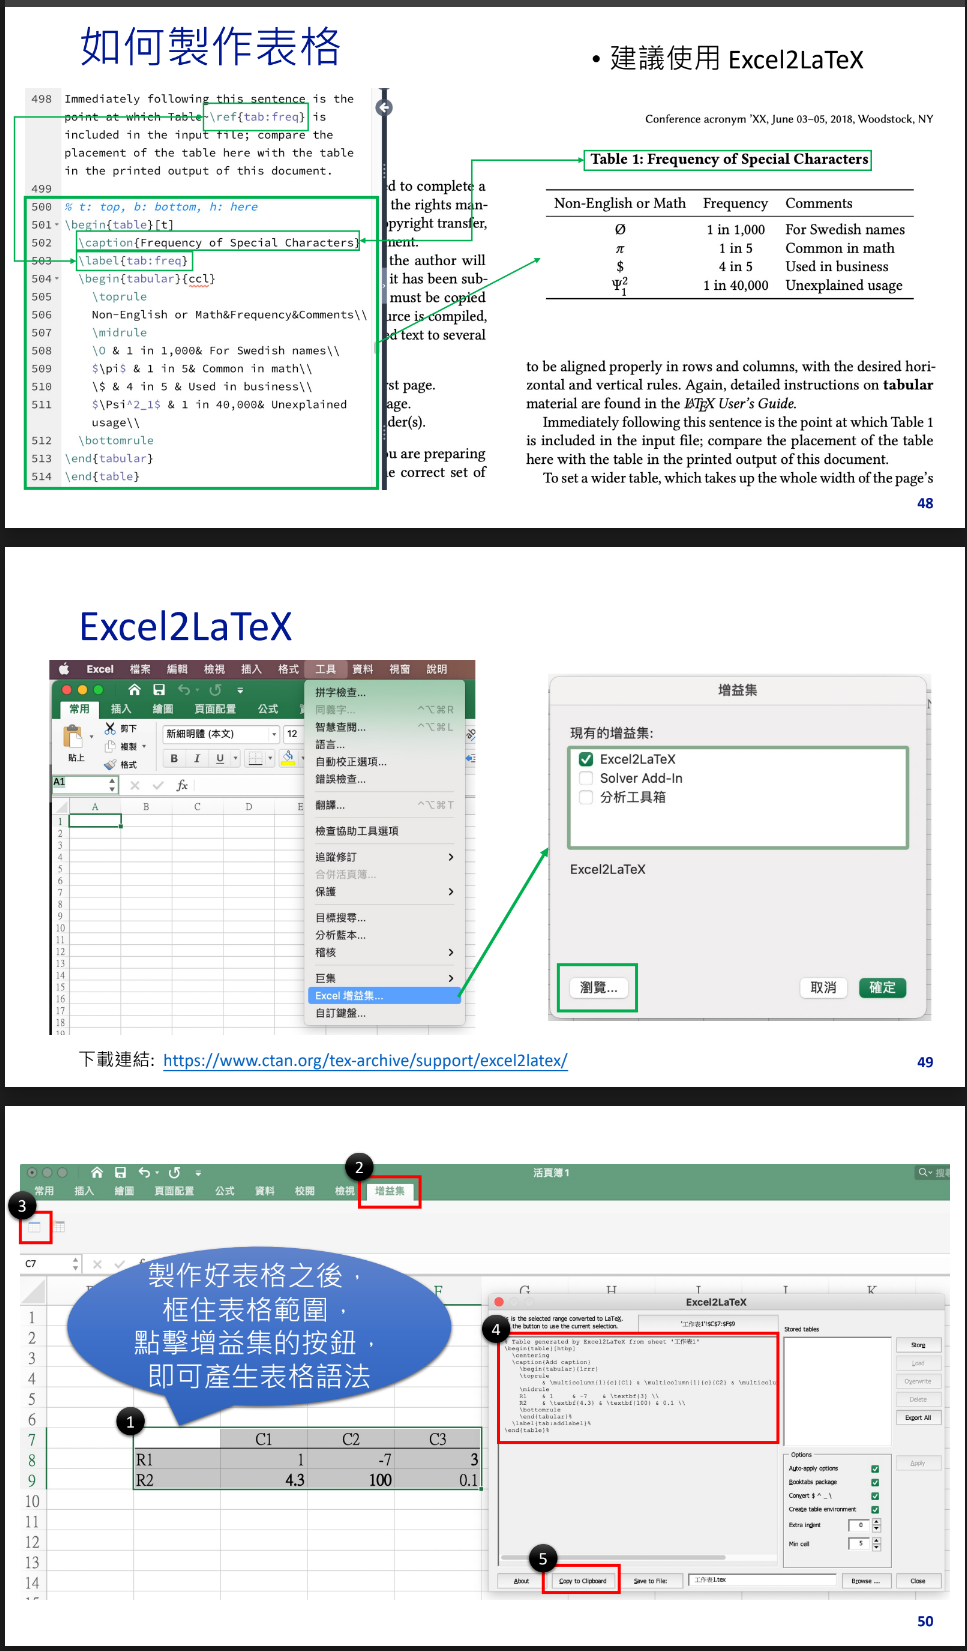
\includegraphics[width=0.8\textwidth]{img/excel2latex.png}
	\caption{Excel2LaTeX.}
	\label{fig:excel2latex}
\end{figure}

 \newpage
\chapter{Data Fusion Algorithm}
\label{ch:method}

\begin{figure}[htb]
	\centering
	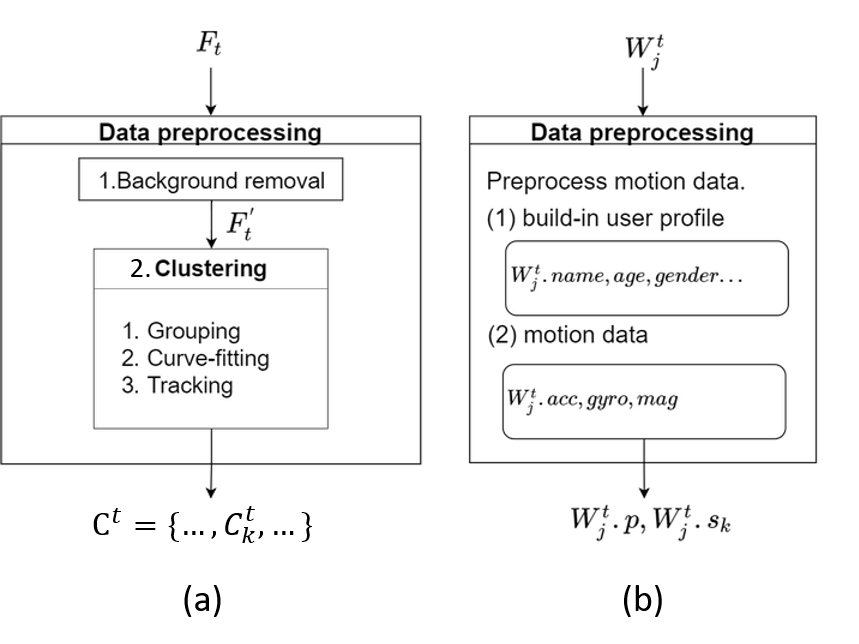
\includegraphics[width=0.6\textwidth]{img/data_preprocessing.png}
	\caption{An example for putting figure.}
	\label{fig:model}
	\vspace{-10mm}
\end{figure}

\section{Data Preprocessing}
\label{sec:SMA}
An example for section. Both LiDAR and wearable sensors will generate continuous data to our fusion server. Fig~\ref{fig:model} shows how these raw data are preprocessed. 


\subsection{2D LiDAR Data}
An example for subection. The LiDAR data preprocessing contains two parts: (i) background removal and (ii) clustering. Background removal 
....

 \newpage
\chapter{Performance Evaluation}
\label{ch:evaluation}

In this section, 整理效能評估.

下面是subfigure的範例 (其實我個人不常用這個語法, 我都直接在繪圖工具上把圖片整合在一起 XD)

\begin{figure}
     \centering
     \begin{subfigure}[]{0.3\textwidth}
         \centering
         
\includegraphics[width=\textwidth]{img/fig1.png}
         \caption{figure 1}
         \label{fig:11111}
     \end{subfigure}
     \hfill
     \begin{subfigure}[]{0.3\textwidth}
         \centering
         
\includegraphics[width=\textwidth]{img/fig2.png}
         \caption{figure 2}
         \label{fig:22222}
     \end{subfigure}
     \hfill
     \begin{subfigure}[]{0.3\textwidth}
         \centering
         
\includegraphics[width=\textwidth]{img/fig3.png}
         \caption{figure 3}
         \label{fig:33333}
     \end{subfigure}
        \caption{Three simple graphs}
        \label{fig:three graphs}
\end{figure} \newpage
\chapter{Conclusions}
\label{ch:conclusion}
Write your conclusion here.
 
 \newpage


% ====================================================
% 13. 參考文獻 Reference (檔案名稱 ref.bib)
%\ClearShipoutPicture % 把ref的浮水印關掉


\phantomsection
\iftoggle{toc-use-cn} % 使用中文
{\addcontentsline{toc}{chapter}{參考文獻}
\renewcommand{\bibname}{參考文獻}} 
{\addcontentsline{toc}{chapter}{References}
\renewcommand{\bibname}{References}
} 


\bibliographystyle{IEEEtran}
\bibliography{ref}


% 14. 附錄 Appendix (有需要再刪除註解 & 編輯該檔案)
%\titleformat{\chapter}{\normalfont\huge\bfseries}{}{1em}{}

\chapter{Appendix 附錄}
\label{ch:appendix}

附錄資料
 \newpage


% =========================================
% [113年2月19日後上傳圖書館博碩士論文系統者適用] 
% 15. 學位論文發表形式確認書
% 16. 著作彙編之學位論文資訊及彙編學術著作之共同作者貢獻聲明書
% 這兩個不用附在論文PDF檔裡面

% 說明1: https://aa.nycu.edu.tw/userfiles/aach/files/20240125111443441.pdf
% 說明2: "國立陽明交通大學著作彙編之學位論文應行注意事項" https://bit.ly/457NTHk

% [心得感想]
% 畢業論文有使用到"就學期間發表"的論文, 就要填寫. 畢業後才刊登論文, 就屬於"不是".
% 對博士生來說, 在學期間可能發表很多篇論文, 可以放在畢業論文裡, 只是要記得填寫著作彙編的表格. 

% 著作彙編的說明
% https://ethics.moe.edu.tw/resource/epaper/html/27/


\balance
\end{document}
